% Options for packages loaded elsewhere
\PassOptionsToPackage{unicode}{hyperref}
\PassOptionsToPackage{hyphens}{url}
%
\documentclass[
  9pt,
  ignorenonframetext,
]{beamer}
\usepackage{pgfpages}
\setbeamertemplate{caption}[numbered]
\setbeamertemplate{caption label separator}{: }
\setbeamercolor{caption name}{fg=normal text.fg}
\beamertemplatenavigationsymbolsempty
% Prevent slide breaks in the middle of a paragraph
\widowpenalties 1 10000
\raggedbottom
\setbeamertemplate{part page}{
  \centering
  \begin{beamercolorbox}[sep=16pt,center]{part title}
    \usebeamerfont{part title}\insertpart\par
  \end{beamercolorbox}
}
\setbeamertemplate{section page}{
  \centering
  \begin{beamercolorbox}[sep=12pt,center]{part title}
    \usebeamerfont{section title}\insertsection\par
  \end{beamercolorbox}
}
\setbeamertemplate{subsection page}{
  \centering
  \begin{beamercolorbox}[sep=8pt,center]{part title}
    \usebeamerfont{subsection title}\insertsubsection\par
  \end{beamercolorbox}
}
\AtBeginPart{
  \frame{\partpage}
}
\AtBeginSection{
  \ifbibliography
  \else
    \frame{\sectionpage}
  \fi
}
\AtBeginSubsection{
  \frame{\subsectionpage}
}
\usepackage{amsmath,amssymb}
\usepackage{lmodern}
\usepackage{iftex}
\ifPDFTeX
  \usepackage[T1]{fontenc}
  \usepackage[utf8]{inputenc}
  \usepackage{textcomp} % provide euro and other symbols
\else % if luatex or xetex
  \usepackage{unicode-math}
  \defaultfontfeatures{Scale=MatchLowercase}
  \defaultfontfeatures[\rmfamily]{Ligatures=TeX,Scale=1}
\fi
% Use upquote if available, for straight quotes in verbatim environments
\IfFileExists{upquote.sty}{\usepackage{upquote}}{}
\IfFileExists{microtype.sty}{% use microtype if available
  \usepackage[]{microtype}
  \UseMicrotypeSet[protrusion]{basicmath} % disable protrusion for tt fonts
}{}
\makeatletter
\@ifundefined{KOMAClassName}{% if non-KOMA class
  \IfFileExists{parskip.sty}{%
    \usepackage{parskip}
  }{% else
    \setlength{\parindent}{0pt}
    \setlength{\parskip}{6pt plus 2pt minus 1pt}}
}{% if KOMA class
  \KOMAoptions{parskip=half}}
\makeatother
\usepackage{xcolor}
\IfFileExists{xurl.sty}{\usepackage{xurl}}{} % add URL line breaks if available
\IfFileExists{bookmark.sty}{\usepackage{bookmark}}{\usepackage{hyperref}}
\hypersetup{
  pdftitle={Surrogate Optimization:Space-Filling Designs},
  pdfauthor={BIOE 498/598 PJ},
  hidelinks,
  pdfcreator={LaTeX via pandoc}}
\urlstyle{same} % disable monospaced font for URLs
\newif\ifbibliography
\setlength{\emergencystretch}{3em} % prevent overfull lines
\providecommand{\tightlist}{%
  \setlength{\itemsep}{0pt}\setlength{\parskip}{0pt}}
\setcounter{secnumdepth}{-\maxdimen} % remove section numbering
\usepackage{tikz}
\usepackage{booktabs}
\renewcommand\mathfamilydefault{cmr}
\usetikzlibrary{positioning,shapes.misc,calc,backgrounds,scopes}
\ifLuaTeX
  \usepackage{selnolig}  % disable illegal ligatures
\fi

\title{Surrogate Optimization:\newline Space-Filling Designs}
\author{BIOE 498/598 PJ}
\date{Spring 2021}

\begin{document}
\frame{\titlepage}

\begin{frame}{From local to global optimization}
\protect\hypertarget{from-local-to-global-optimization}{}
\begin{itemize}
\tightlist
\item
  Steepest Ascent/RSM finds the optimal operating conditions in a
  \textbf{local} design space.
\item
  It's possible a better operating condition exists far away.
\item
  \textbf{Global optimization} searches the entire design region.
\end{itemize}

\bigskip
\pause
\begin{center}
  \begin{tabular}{llll}
    \toprule
    \textbf{Method} & \textbf{Search} & \textbf{\# of samples} & \textbf{Sampling} \\
    \midrule
    Steepest Ascent/RSM & local & 10--100's & very expensive, noisy \\
    Surrogate Optimization & global & 100--1000's & moderately expensive \\
    Reinforcement Learning & global & 10,000$+$ & very inexpensive \\
    \bottomrule
  \end{tabular}
\end{center}
\end{frame}

\begin{frame}{Surrogate Optimization}
\protect\hypertarget{surrogate-optimization}{}
\begin{itemize}
\tightlist
\item
  Assume we are trying to optimize a function \(f\) that is
  \textbf{expensive} to evaluate.
\item
  Instead, we use evaluations of \(f\) to build a surrogate model
  \(\tilde{f}\) that is \textbf{cheap} to evaluate.
\item
  We optimize \(\tilde{f}\) to find good candidates for evaluation by
  \(f\).
\end{itemize}

\bigskip
\pause

\tikzset{boxed/.style={
  thick,
  draw=black,
  top color=white,
  text height=1.5ex,
  text depth=.25ex
}}

\begin{center}
\begin{tikzpicture}[>=latex]
  \node (start) {};
  \node (design) [boxed, right=2cm of start] {design $X$};
  \node (data) [boxed,right=1.5cm of design] {$y$};
  \node (surrogate) [boxed,right=2cm of data] {surrogate $\tilde{f}$};
  \node (optimal) [boxed,right=0.5cm of surrogate] {$x^*$};
  \draw [->] (start) -- (design) node [midway,above] {space-filling};
  \draw [->] (design) -- (data) node [midway,above] {$f(X)$};
  \draw [->] (data) -- (surrogate) node [midway,above] {$\mathcal{GP}(X,y)$};
  \draw [->] (surrogate) -- (optimal);
  \draw [->] (surrogate.south) -- ++(0,-0.5) -| (design.south) node [near start,below] {sequential design};
\end{tikzpicture}
\end{center}
\end{frame}

\begin{frame}{Why use surrogates?}
\protect\hypertarget{why-use-surrogates}{}
\begin{center}
  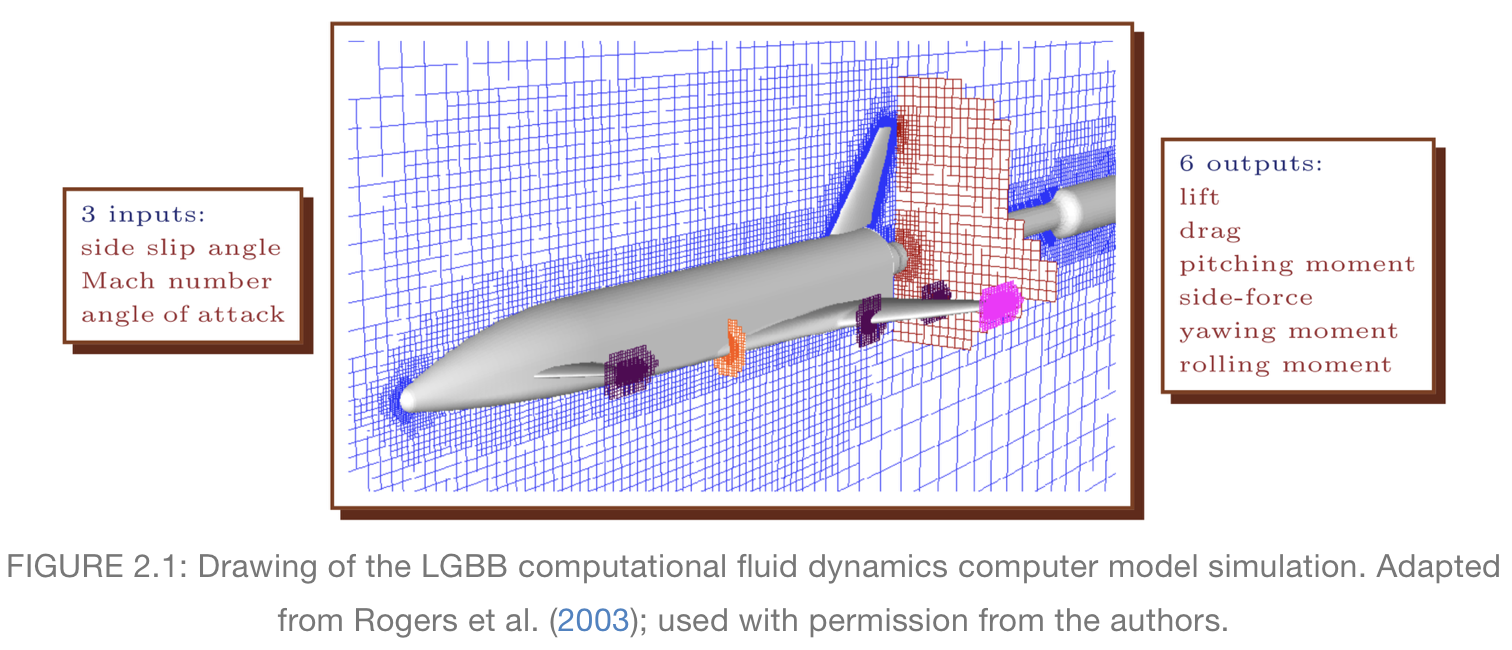
\includegraphics[width=\textwidth]{figures/rocketbooster.png}
\end{center}
\end{frame}

\begin{frame}{Surrogate optimization by many names}
\protect\hypertarget{surrogate-optimization-by-many-names}{}
\begin{itemize}
\tightlist
\item
  \textbf{Computer experiments}, \textbf{emulation}, or
  \textbf{metamodeling} based on historical usage.
\item
  \textbf{Kriging} from geostatistics (refers to prediction with GPR).
\item
  \textbf{Nonparametric Bayesian optimization} to impress your manager.
\item
  \textbf{Sequential design} in the DOE field.
\item
  \textbf{Active learning} in the ML field.
\end{itemize}
\end{frame}

\begin{frame}{Today: Space-Filling Designs}
\protect\hypertarget{today-space-filling-designs}{}
\begin{itemize}
\tightlist
\item
  Global optimization requires data from every part of the design space.
\item
  We want to cover as much of the space as possible with the fewest
  number of points.
\item
  \textbf{Space-Filling Designs} spread samples over a multidimensional
  space \([0,1]^k\).

  \begin{itemize}
  \tightlist
  \item
    Other design spaces can be rescaled to match this hypercube.
  \end{itemize}
\item
  Later we will use the surrogate to \emph{intelligently} augment the
  initial design.
\end{itemize}
\end{frame}

\begin{frame}{How about evenly-spaced designs (grids)?}
\protect\hypertarget{how-about-evenly-spaced-designs-grids}{}
\begin{columns}
\begin{column}{0.6\textwidth}

Evenly-spaced designs have two big drawbacks:
\medskip
\begin{enumerate}
  \onslide<2->{
    \item Regular spacing can alias patterns in the response surface.
    \begin{center}
      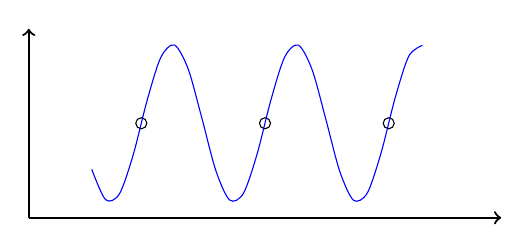
\begin{tikzpicture}
          \draw [->,thick] (-3,-1.2) -- (3,-1.2);
          \draw [->,thick] (-3,-1.2) -- (-3,1.2);
          \draw (0,0) circle (2pt) +(-1.571,0) circle (2pt) +(1.571,0) circle (2pt);
          \onslide<3->{
            \draw[domain=-2.2:2, smooth, variable=\x, blue] plot ({\x}, {sin(4*\x r)});
          }
      \end{tikzpicture}
    \end{center}
  }
  \item<4-> Regular designs have poor \textbf{projection spacing}. This is a problem because of effect sparsity!
\end{enumerate}

\end{column}
\begin{column}{0.4\textwidth}

\begin{center}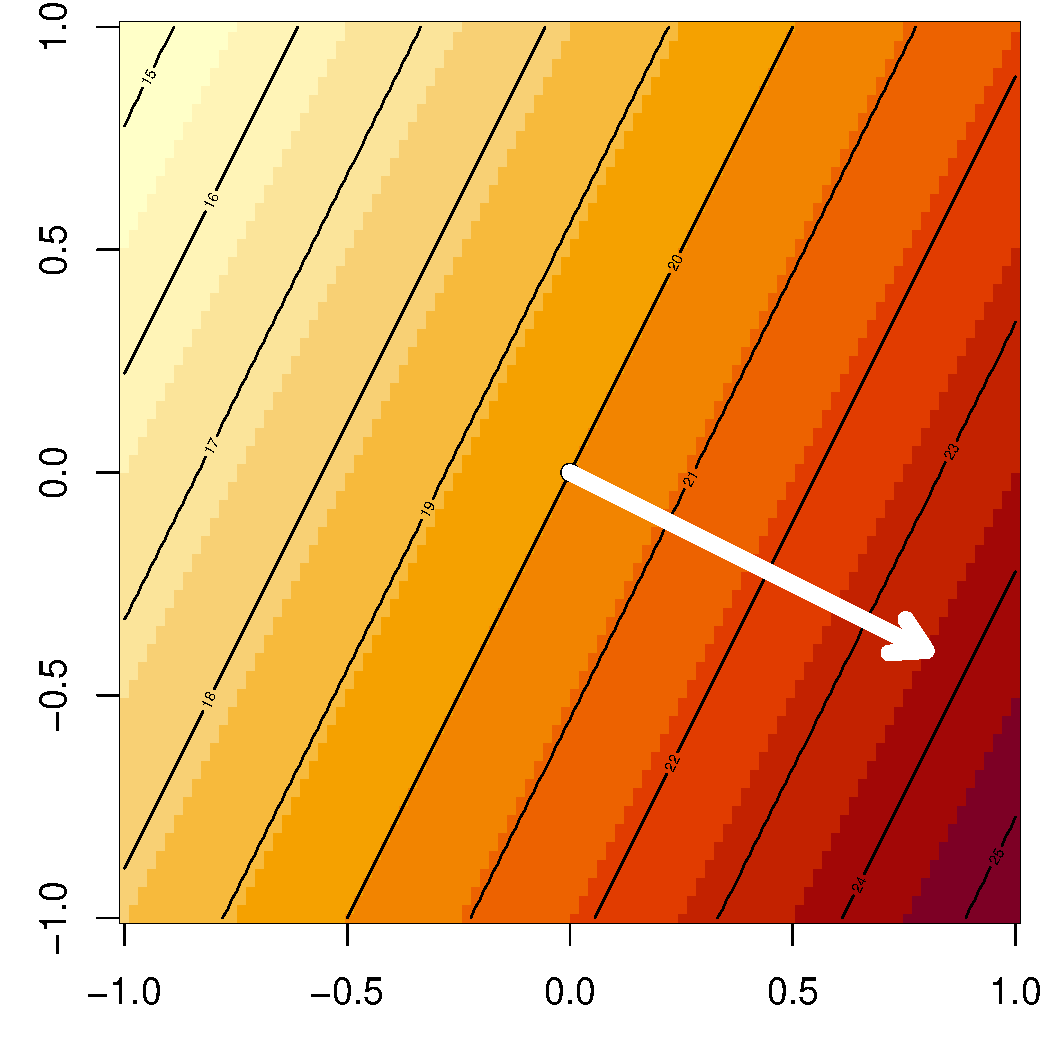
\includegraphics{22_SpaceFillingDesigns_files/figure-beamer/unnamed-chunk-1-1} \end{center}
\end{column}
\end{columns}
\end{frame}

\begin{frame}{Why not random locations?}
\protect\hypertarget{why-not-random-locations}{}
People often overestimate the randomness of random processes. Take our
``random'' string of digits as an example. How many repeated digits did
you find in your sequence?

\pause

\begin{center}\includegraphics{22_SpaceFillingDesigns_files/figure-beamer/unnamed-chunk-2-1} \end{center}
\end{frame}

\begin{frame}{Random designs are ``clumpy''}
\protect\hypertarget{random-designs-are-clumpy}{}
\begin{columns}
\begin{column}{0.6\textwidth}

\onslide<2->{
  We need a \textbf{Space-Filling Design} that
  \medskip
  \begin{enumerate}
    \item Places points semi-randomly to avoid aliasing
    \item Avoids "clumps" of points
    \item Projects well onto lower dimensions
  \end{enumerate}
}

\end{column}
\begin{column}{0.4\textwidth}

\begin{center}\includegraphics{22_SpaceFillingDesigns_files/figure-beamer/unnamed-chunk-3-1} \end{center}

\end{column}
\end{columns}
\end{frame}

\begin{frame}{Latin Hypercube Designs}
\protect\hypertarget{latin-hypercube-designs}{}
\begin{columns}
\begin{column}{0.6\textwidth}

A Latin Hypercube Design (LHD) is a semi-random design that guarantees uniform projection.

\medskip
\begin{itemize}
  \item Each dimension is divided into $n$ intervals.
  \item Points are placed randomly, but only one point is allowed in each interval along each dimension.
  \item Points can be placed in the center or a random position in each "square".
  \item LHDs are like a simplified Sudoku puzzle!
\end{itemize}

\end{column}
\begin{column}{0.4\textwidth}

\onslide<1->{

\begin{center}\includegraphics{22_SpaceFillingDesigns_files/figure-beamer/unnamed-chunk-4-1} \end{center}
}

\medskip
\onslide<2>{

\begin{center}\includegraphics{22_SpaceFillingDesigns_files/figure-beamer/unnamed-chunk-5-1} \end{center}
}

\end{column}
\end{columns}
\end{frame}

\begin{frame}{Building a LHD}
\protect\hypertarget{building-a-lhd}{}
\begin{columns}
\begin{column}{0.6\textwidth}

\begin{enumerate}
  \item The interval along the first dimension is simply $1\ldots n$; there is no need to randomize.
  \item For each subsequent dimension, select a random permutation of $\{1\ldots n\}$
\end{enumerate}

\bigskip
\begin{center}
  \begin{tabular}{ccc}
    \toprule
    $x_1$ & $x_2$ \\
    \midrule
    1 & 2 \\
    2 & 8 \\
    3 & 1 \\
    4 & 7 \\
    5 & 5 \\
    6 & 4 \\
    7 & 9 \\
    8 & 3 \\
    9 & 6 \\
    \bottomrule
  \end{tabular}
\end{center}

\end{column}
\begin{column}{0.4\textwidth}


\begin{center}\includegraphics{22_SpaceFillingDesigns_files/figure-beamer/unnamed-chunk-6-1} \end{center}

\end{column}
\end{columns}
\end{frame}

\begin{frame}{Beware of randomness (again)}
\protect\hypertarget{beware-of-randomness-again}{}
\begin{columns}
\begin{column}{0.5\textwidth}


\begin{center}\includegraphics{22_SpaceFillingDesigns_files/figure-beamer/unnamed-chunk-7-1} \end{center}
\bigskip
The above design is a LHD, but it is not very random. Rarely we can get permutations that do not space-fill.

\end{column}
\begin{column}{0.5\textwidth}
\onslide<2->{

\begin{center}\includegraphics{22_SpaceFillingDesigns_files/figure-beamer/unnamed-chunk-8-1} \end{center}
\bigskip
One alternative is an Orthogonal Array LHD.
}
\end{column}
\end{columns}
\end{frame}

\begin{frame}{Another option: Maximin Designs}
\protect\hypertarget{another-option-maximin-designs}{}
What we really want is to maximize the distance between the points in
the final design. We can achieve this directly via optimization.

\pause

The \emph{Euclidean distance} between any two points \(x\) and \(x'\) is
\[ d(x,x') = \lVert x-x' \rVert^2 = \sum_{j=1}^k(x_j-x_j')^2 \]

\pause

The \emph{maximin} design matrix with \(n\) samples, called \(X_n\) is
\[ \arg \max_{X_n} \min\{ d(x,x'), \forall x\ne x' \} \]

\pause

Computationally, we begin with a random set of \(n\) points and
iteratively move points until a local optimum is found.
\end{frame}

\begin{frame}[fragile]{The \texttt{maximin} package}
\protect\hypertarget{the-maximin-package}{}
The \texttt{maximin} package creates sequential space-filling designs.
\bigskip

\begin{columns}
\begin{column}{0.5\textwidth}
\texttt{X1 <- maximin::maximin(\\$\quad\quad\quad\quad$n=9, p=2, T=100)\\$\quad$}
\bigskip

\begin{center}\includegraphics{22_SpaceFillingDesigns_files/figure-beamer/unnamed-chunk-9-1} \end{center}
\end{column}
\onslide<2->{
  \begin{column}{0.5\textwidth}
  \texttt{X1 <- maximin::maximin(\\$\quad\quad\quad\quad$n=5, p=2, T=100,\\$\quad\quad\quad\quad$ Xorig=X1\$Xf)}
  \bigskip

\begin{center}\includegraphics{22_SpaceFillingDesigns_files/figure-beamer/unnamed-chunk-10-1} \end{center}
  \end{column}
}
\end{columns}

\bigskip
\onslide<1->{
  \begin{center}
    \footnotesize{\texttt{n}=number of samples, \texttt{p}=number of dimensions, \texttt{T}=number of iterations for the optimizer.}
  \end{center}
}
\end{frame}

\begin{frame}{Summary}
\protect\hypertarget{summary}{}
\begin{itemize}
\tightlist
\item
  Surrogate optimization begins with a space-filling design.
\item
  Grid and random designs are not good.
\item
  LHD and Maximin designs spread points globally and project well to
  lower dimensions.
\item
  \textbf{Next time:} Building a surrogate model from an initial
  space-filling design.
\end{itemize}
\end{frame}

\end{document}
